\documentclass[../tp2.tex]{subfiles}

\begin{document}
Uma \textit{Mandatory Access Control} (MAC), ou em português, um controlo de acessos obrigatório é um tipo de política que corresponde a atribuir os direitos de acesso baseados nos regulamentos da organização. Este tipo de políticas assentam no facto da informação pertencer à organização e não ser apenas de carácter individual, sendo assim da competência da organização garantir o controlo da política de segurança. Este tipo de políticas esforça-se para combater e evitar ataques do tipo cavalo de Troia. \par 
A forma de restringir o acesso de utilizadores a objetos baseia-se numa \textit{label} com a informação dos dados contidos nos objetos e do nível de autorização dos utilizadores a informação dessa sensibilidade.\par 
Estas diferentes \textit{labels} são então dispostas numa espécie de grafo, \textit{lattice} onde é necessário garantir a dominância entre diferentes \textit{labels}, ou seja, \textit{labels} de um nível superior têm de ser de um nível de segurança mais restrito e conter a informação da \textit{label} abaixo. Em termos matemáticos, esta dominância pode ser exemplificada da seguinte forma:\par 
Tendo duas \textit{labels} diferentes, $L1 = (S1,C1)$ e $L2 = (S2,C2)$, se tivermos que $L1 \leq L2 $, significando que $L1$ não é mais restritivo que $L2$ e que $C1 \subseteq C2$, fica claro que \textit{label} $L2$ tem então dominância sobre a \textit{label} $L1$.\par 
Neste trabalho prático, é pedido que na construção da \textit{lattice} se tenha em conta que os professores são classificado com a \textit{label} \texttt{(C,\{AS,ScS\})} e os alunos com a \textit{label} \texttt{(C,\{AS\})}, sendo que existem três níveis de segurança, \textbf{P} para o nível Público, \textbf{C} para o nível Confidencial e por último \textbf{SC} para \textit{Strictly Confidential}, com as categorias \textbf{AS} para os Serviços Académicos e \textbf{ScS} para os serviços científicos.
Com isto em mente, a \textit{lattice} criada para este trabalho prático está demonstrada na Figura \ref{fig:lattice}.

\begin{figure}[H]\centering \captionsetup{justification=centering,margin=2cm} \centerline{\includegraphics[scale=0.6]{../imagens/lattice.png}} \caption{\textit{Lattice} criada neste trabalho prático.} \label{fig:lattice}

\end{figure}

No diagrama anterior podemos verificar a existência destas dominâncias entre diferentes \textit{labels}. Por exemplo a \textit{label} \texttt{(SC,\{AS,ScS\})} é dominante sobre as \textit{labels} \texttt{(SC,\{ScS\})}, \texttt{(SC,\{AS\})} e \texttt{(C,\{AS,ScS\})}. A \textit{label} \texttt{(SC,\{AS,ScS\})} acaba por ser dominante sobre todas as restantes \textit{labels} por consequência da demonstração anterior. Como este trabalho é desenvolvido no contexto universitário, podemos dizer que a \textit{label} com dominância sobre as restantes poderia ser o Reitor da Universidade, por exemplo.\par 
É importante notar que as regras de controlo da informação são garantidas. Seja $L(x)$ a \textit{label} da relação $x$, um utilizador \textit{U} apenas pode ler ficheiros \textit{F} se $L(F) \leq L(U)$, ou seja, os utilizadores não conseguem ``ler para cima''. Um utilizador \textit{U} poderá escrever num ficheiro \textit{F} apenas se $L(U) \leq L(F)$, ou seja, os utilizadores não podem ``escrever para baixo''.\par 
De forma a compreender visualmente este tipo de regras, temos na Figura \ref{fig:regras} um exemplo com quatro nível de segurança, \textbf{TS} para \textit{Top-Secret}, \textbf{S} para \textit{Secret}, \textbf{C} para \textit{Classified} e por fim \textbf{U} para \textit{Unclassified}.

\begin{figure}[H]\centering \captionsetup{justification=centering,margin=2cm} \centerline{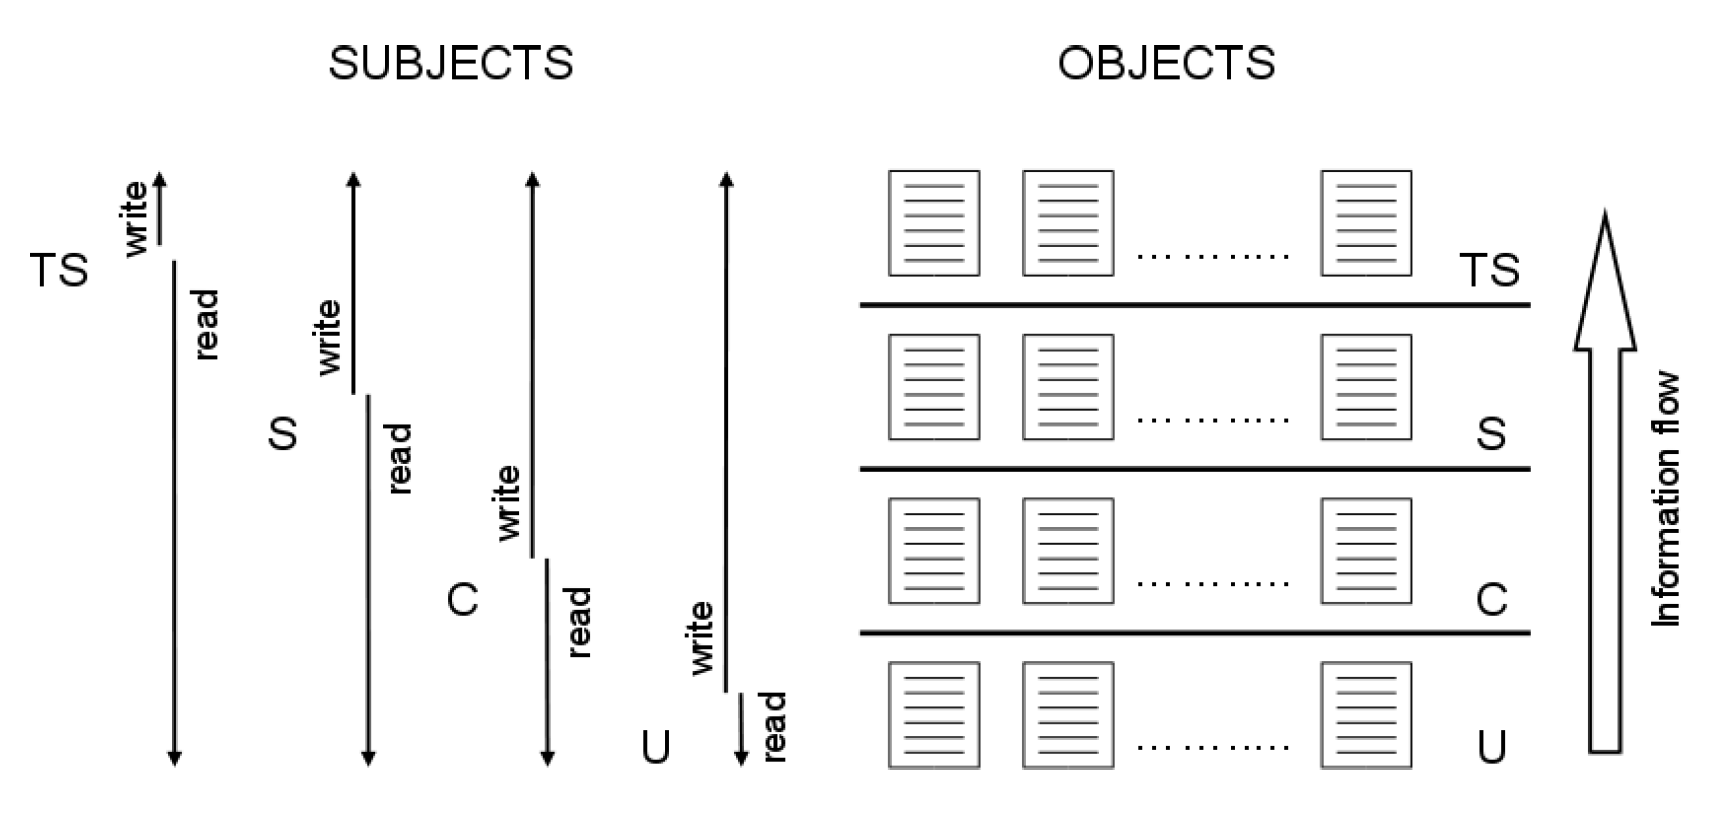
\includegraphics[scale=0.4]{../imagens/regras.png}} \caption{Regras que estabelecem a \textit{Mandatory Access Control}.} \label{fig:regras}

\end{figure}
\end{document}